\begin{center}
    \vspace{5cm}
    {\Huge\textbf{\section{\underline{Decisions}}}} % Large and bold text
    \begin{figure}[h]
        \centering
        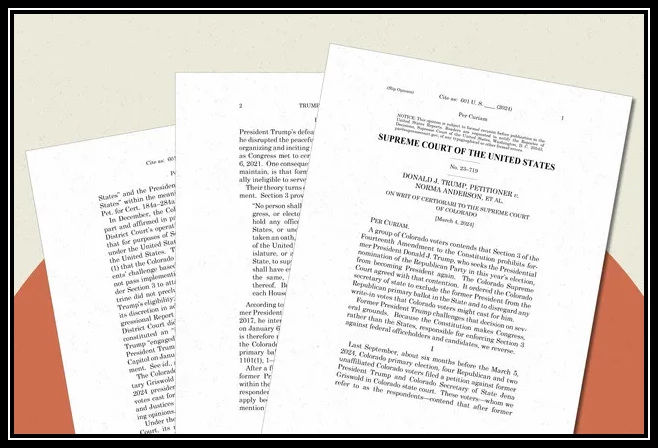
\includegraphics[width=0.7\textwidth]{Figures/intro_page_images/decision_image_1.jpg} \\
        \footnotesize{Photo Credit: POLITICO Illustration (Politico)} \\
        \vspace{2mm}
        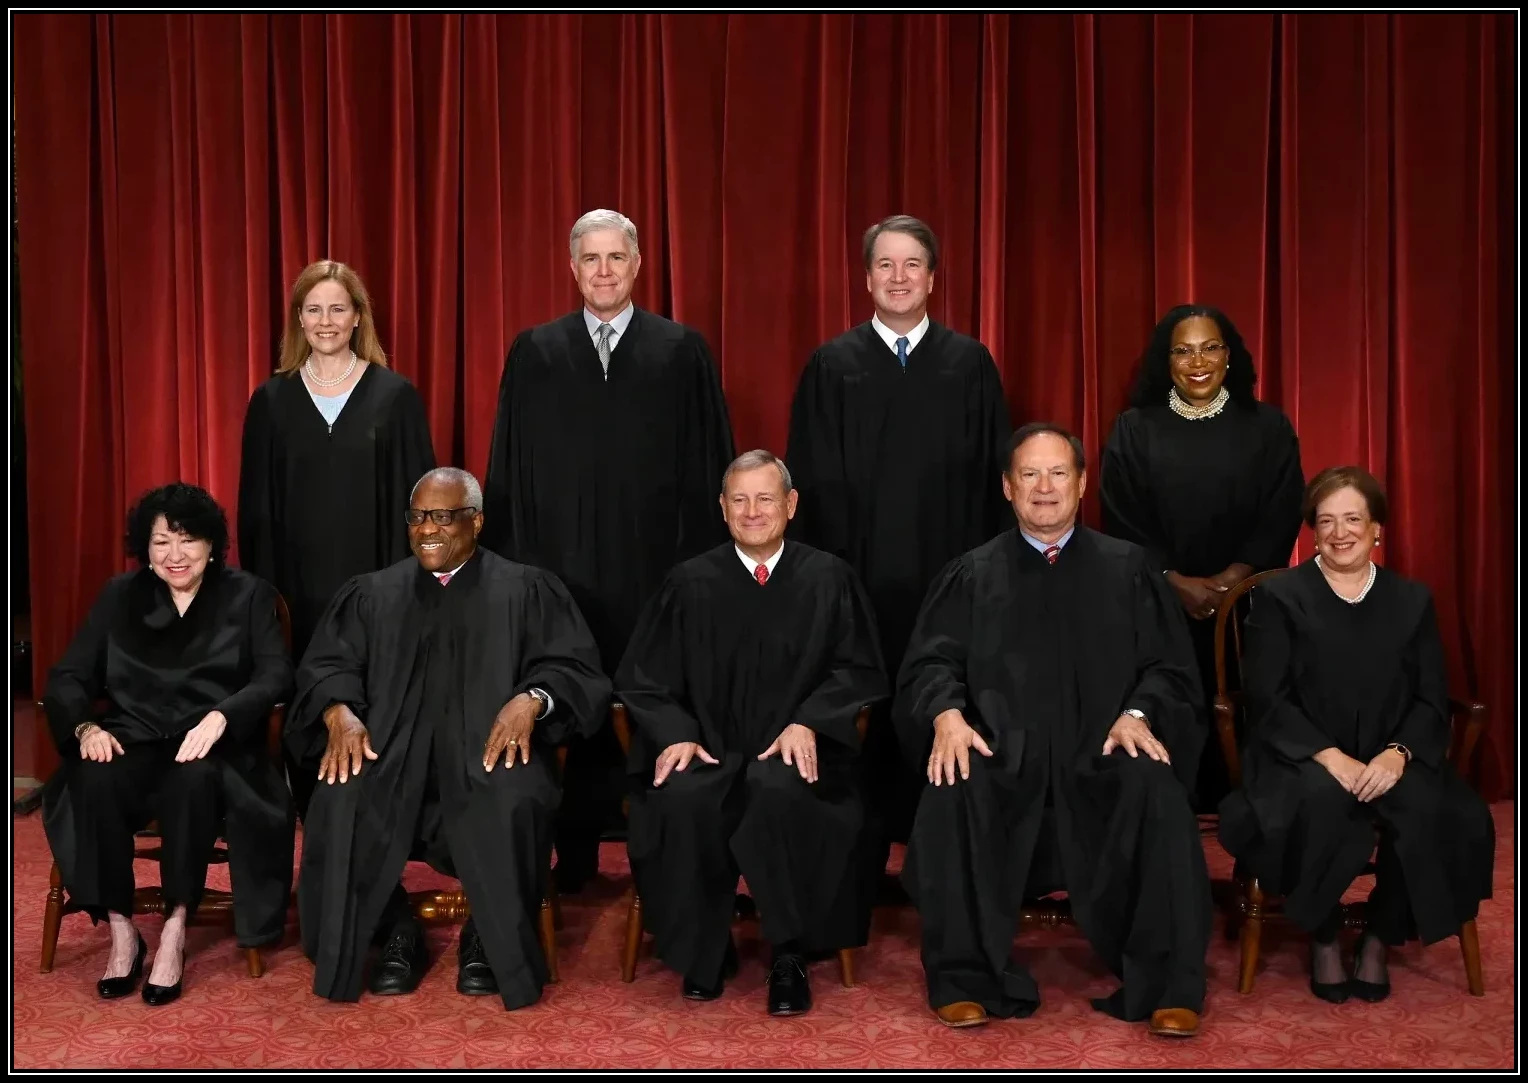
\includegraphics[width=0.7\textwidth]{Figures/intro_page_images/decision_image_2.jpg} \\
        \footnotesize{Photo Credit: Olivier Douliery (AFP via Getty Images file)} \\

    \end{figure}
\end{center}

\newpage

\begin{center}

\begin{table}[H]
    \centering
    \caption{What's Included (Decisions)}
    \label{tab:example}
    \vspace{1mm}
    \begin{tabularx}{\textwidth}{>{\centering\arraybackslash}p{0.33\textwidth}>{\centering\arraybackslash}X}
        \toprule
        Topic & Description \\
        \midrule
        Justice Agreement Matrix & \RaggedRight Percentage of decisions where Justices coalesced similarity -- i.e., were \emph{both} in Majority or Dissent (ex: Justices Alito and Sotomayor) \\
        \addlinespace
        Decision Overviews & \RaggedRight 2023 Term Decisions organized by sitting (month) with corresponding summary of case-level issue, docket number, holding, opinion author, and coalition size. \\
        \addlinespace
        Circuit Scorecard & \RaggedRight Percentage of \emph{Affirmed} and \emph{Reversed} (and/or \emph{Vacated}/\emph{Remanded}) decisions by U.S. Circuit Courts of Appeals. \\
        \addlinespace
        Decisions by Coalition and Term & \RaggedRight Summary of decisions by coalition size between 2018 and 2023 Terms. \\
        \addlinespace
        Share of Cases Decided (9-0) by Term & \RaggedRight Percentage of cases decided (9-0) between 2018 and 2023 Terms. \\
        %\addlinespace
        %Share of Cases with Filed Dissent or Concurrence by Term & \RaggedRight Percentage of cases where a dissent or concurrence was filed between 2018 and 2023 Terms. \\
        \addlinespace
        Opinion Lengths & \RaggedRight Top-10 Longest and Shortest Opinions of 2023 Term. \\
        \addlinespace
        Decision Turnover & \RaggedRight Average number of days elapsed between oral arguments \& decision by the Court (organized by argument sitting and term).\\
        \addlinespace
        Frequency in Majority by Term & \RaggedRight Percentage of cases where each Justice was in the majority between 2005 and 2023 Terms (Roberts Court). \\
        \addlinespace
        Ideological Splits & \RaggedRight Share of (6-3) and (5-3) cases between OT2020 and OT2023 where the Court was ideologically split. \\
        \addlinespace
        Opinion Authorship & \RaggedRight Share of opinions -- Majority, Concurrences (Regular, In Judgement, or In Part), and Dissents -- authored by each Justice. \\
        \bottomrule
    \end{tabularx}
\end{table}
\end{center}

\newpage

\begin{center}
\vspace{5mm}
\Huge\textbf{\subsection{\underline{Note on Decision Coding}}}
\end{center}

\noindent We recognize that the array of potential case-level votes do not always neatly align with a definitive indicator that a Justice should be considered a member of the Majority or Minority (\emph{Dissenting}) coalition. In particular, votes by Justices \emph{Concurring and Dissenting In Part}, \emph{Concurring in Judgement}, joining (and/or authoring) several concurrences, etc., are not as clear of an indicator as authoring or simply joining the majority. These special votes could lead to varying records of majority and minority coalitions sizes depending on the source. For example, a decision rendered with a single Justice authoring an opinion \emph{Concurring In Part, and Dissenting in Part} could reasonbly be coded as either (9-0) or (8-1), given that the Justice neither fully joined -- nor fully dissented -- from the Court's majority opinion. \\

To maintain methodological consistency, we code choices to join the \textbf{Minority} (\emph{Dissent}) as instances where a Justice (1) Authored a Dissenting Opinion or (2) \textbf{Only} Joined a Dissenting Opinion. Below we list the cases impacted by this coding scheme. \\

\begin{itemize}

\item \emph{Acheson Hotels LLC v. Laufer} (22-429) -- Decided 12/05/2023
\item \emph{Trump v. Anderson} (23-719) -- Decided 03/04/2024
\item \emph{Muldrow v. City of St. Louis} (22-193) -- Decided 04/17/2024
\item \emph{Vidal v. Ester} (23-704) -- Decided 06/13/2024
\item \emph{Starbucks Corp. v. McKinney} (23-367) -- Decided 06/13/2023
\item \emph{Moore v. United States} (22-800) -- Decided 06/20/2024
\item \emph{Department of State v. Munoz} (23-334) -- Decided 06/21/2024
\item \emph{Smith v. Arizona} (22-899) -- Decided 06/21/2024
\item \emph{Moyle v. United States} (23-726) -- Decided 06/27/2024
\item \emph{Moody v. NetChoice} (22-277) -- Decided 07/01/2024
\item \emph{Trump v. United States} (23-939) -- Decided 07/01/2024
\end{itemize}

\newpage

\begin{center}
\vspace{5mm}
\Huge\textbf{\subsection{\underline{Additional Notes: Opinion Consolidations}}}
\end{center}

\begin{itemize}

\item Given the post-argument consolidation of \emph{Loper Bright Enterprises v. Raimondo} (22-451) with \emph{Relentless, Inc., et al. v. Department of Commerce} (22-1219), we report the outcome collectively under \emph{Loper Bright} as (6-3) with Justice Jackson joining Justice Sotomayor's dissent (though Justice Jackson did not participate in the proceedings of 22-451).
\item Given the post-argument consolidation of \emph{Moody v. NetChoice, LLC} (22-277) with \emph{Netchoice, LLC v. Paxton} (22-555), we report the outcome collectively under \emph{Moody v. Net Choice} as (9-0) with Justice Kagan authoring.

\end{itemize}




